
%%
%% Submission requirements
%% 12 pages + plus as many pages as needed for references.
%%
%% Blind reviewing of full papers will be done by the program committee
%% and external review committee, with limited use of outside
%% referees. Authors must make a good faith effort to anonymize their
%% submissions, and they should not identify themselves either explicitly
%% or by implication (e.g., through the references or
%% acknowledgments). Submissions violating the detailed formatting and
%% anonymization rules will not be considered for publication.


\documentclass[10pt,twocolumn]{article}
\usepackage{times}
\usepackage{fullpage}

% added for our purpose
\usepackage{url}
\usepackage{upgreek}
\newcommand{\microsecond}{$\upmu{}s$}

% debugging only
\newcommand{\edb}[1]{\noindent{\color{Plum} {\bf \fbox{EdB}} {\it#1}}}
\newcommand{\adam}[1]{\noindent{\color{Red} {\bf \fbox{AB}} {\it#1}}}
\newcommand{\christos}[1]{\noindent{\color{Green} {\bf \fbox{CK}} {\it#1}}}
\newcommand{\georgios}[1]{\noindent{\color{Blue} {\bf \fbox{GP}} {\it#1}}}
%\newcommand{\babak}[1]{\noindent{\color{Purple} {\bf \fbox{BF}} {\it#1}}}
\newcommand{\todo}{\noindent $\triangleright $~}



\begin{document}

\title{\bf Title}
\author{Paper \# 123 XXX}
\date{}
\maketitle
\thispagestyle{empty}

%

\begin{abstract}

  Web-scale applications are placing aggressive demands on the
  implementation of the TPC/IP networking stack in modern systems,
  such as high packet rates for small messages, microsecond-scale tail
  latency, support for hundreds of thousands of connections, and
  elastic use of system resources. The conventional wisdom is that
  such requirements are best addressed outside the operating system,
  in a user-level implentation of the networking stack.

  We present {\it IX}, a {\it dataplane operating system} specifically
  designed for web-scale, event-driven applications.  The IX
  architecture separates control plane from the dataplanes and
  provides a native, zero-copy API that explicitly exposes flow
  control to applications. However, IX uses hardware virtualization to
  offer the same protection model as commodity operating systems. IX
  optimizes for both bandwidth and latency by processing bounded
  batches of packets to completion and by eliminating coherence
  traffic and synchronization on multi-core systems. 

  \christos{TBD} We demonstrate that IX outperforms Linux by X for packet rate and by
  Y for latency. IX also outperforms a state-of-the-art, user-space
  networking stack by X for packet rate and by Y for
  latency. Moreover, we show that IX efficiently supports Z
  connections and improves the overall performance of real-world
  applications by a factor of W.

\end{abstract}




\section{Related Work}

\todo need a table that compares us with related work (!)

\todo Improving operating system kernels to scale

\todo Limitations of the POSIX socket API

\todo User-level networking

\todo Protocol offload engines

\todo Energy-proportionality.   Have a graph that shows the energy-proportionality of a dynamic core approach.


\section{Design Principles}

\begin{figure}
\hspace*{-0.25in}\centering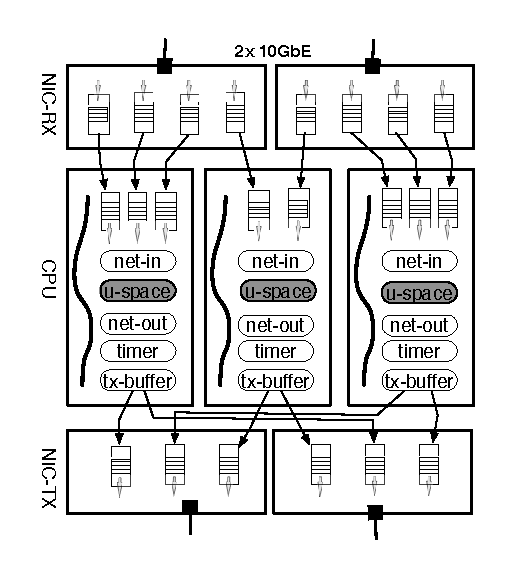
\includegraphics{figs/queues-cores.eps}

\vspace*{-0.25in}\caption{Example of IX scaling across two NICs interfaces, 8 NIC RX queues, and 3 CPU hardware threads.} 

\label{fig:queues-cores}
\end{figure}



\todo Separation of control and data planes

\todo Coherency-free operations  (ala multikernel~\cite{DBLP:conf/sosp/BaumannBDHIPRSS09})

\todo Dynamic spinning cores : re-define pthread abstraction but use it in a different way

\todo Asynchronous channels (like Megapipe)

\todo Abstraction layers: libevent, libpcap


\section{Implementation}

\todo System Archictecture (Dune~\cite{belay2012dune})

\todo Driver layer

\todo TODO (figures, ...)

\section{Evaluation}


\todo Compare apples-to-apples with Megapipe, and mTCP in terms of microbenchmarks.

\todo Baseline comparison of state-of-the art systems include:  Linux (some recent version, with SO\_REUSEPORT); Megapipe (if possible), mTCP (if possible). 

\todo Microbenchmark: short TCP transactions (echo server, as defined in megapipe).   Goal is to beat mTCP (and therefore all others) hands down.

\todo Benchmark: memcached - compare with FB results (?)

\todo Benchmark: lightttpd -- used by Affinity-Accept and mTCP.  

\todo ngnx: an actually used webserver.


\section{Discussion}
\section{Conclusion}





%
\section{Introduction}

Dune~\cite{belay2012dune} ...

%

\section{Related Work}
\label{sec:related}

We organize the discussion topically, while avoiding redundancy with
the commentary already exposed in \S\ref{sec:motivation:current}.


\myparagraph{Virtualization hardware:} Hardware support for
virtualization naturally separates control and execution functions,
e.g., to build type-2 hypervisors
~\cite{DBLP:journals/tocs/BugnionDRSW12,misc/kivity07kvm}, run virtual
appliances~\cite{DBLP:conf/lisa/SapuntzakisBCZCLR03}, or processes
with access to privileged instructions~\cite{belay2012dune}.
Arrakis~\cite{peter2013arrakis,arrakisTR13} uses virtualization
hardware, the Barrelfish
multikernel~\cite{DBLP:conf/sosp/BaumannBDHIPRSS09} for control, and
its own networking stack, to separate the dataplane from the control
plane. \ix is a dataplane operating system that uses Linux for
control, Dune for isolation, a mature networking stack for protocol
processing.


\myparagraph{Library operating systems:}
Exokernels proposed to implement system abstractions via library
operating systems linked in with
applications~\cite{DBLP:conf/sosp/EnglerKO95}, extending the
end-to-end principle~\cite{DBLP:journals/tocs/SaltzerRC84} to the
management of system resources.  Library operating systems typically
run as virtual machines ~\cite{DBLP:journals/tocs/BugnionDGR97},
e.g. to deploy cloud services
~\cite{DBLP:conf/asplos/MadhavapeddyMRSSGSHC13}. The \ix kernel limits
itself to the implementation of protocol stack, allowing applications
to implement their own resource management policies, e.g. via the
\texttt{libevent} compatibility layer.


\myparagraph{User-level networking stacks:} User-level network
stacks~\cite{jeong2014mtcp, marinos2013network, openonload} can
outperform kernel-based implementations through specialization and
elimination of redundant layers and abstractions, but trade-off
performance for a weaker security model.  The \ix dataplane
demonstrates that a specialized networking stack can offer performance
and cooperate with applications without having to weaken security and
isolation properties.
 

\myparagraph{Hardware and protocol specialization:} 
Applications can use a connection-less UDP-based protocol for
scalability~\cite{nishtala2013scaling}.  Latency-sensitive datacenter
applications can use specialized Infiniband adapters to expose RDMA
with $1-3$\microsecond latencies to
applications~\cite{DBLP:conf/sosp/OngaroRSOR11,Jose:2011:MDH,mitchell:rdma,dragojevic14farm}.
Specialized FGPAs can replace conventional servers for important
applications such as
memcached~\cite{DBLP:conf/fpga/ChalamalasettiLWARM13}.  \ix is
designed to allow TCP/IP to scale with architectural trends by
elminating kernel bottlenecks.


\myparagraph{Asynchronous and zero-copy interactions:} 
Systems with asynchronous, batched, or exception-less system calls
substantially reduce the overheads associated with frequent kernel
transitions and context switches~\cite{
  soares2010flexsc,han2012megapipe,rizzo2012netmap,jeong2014mtcp}.
Zero-copy reduce data movement overheads and simplifies resource
management~\cite{DBLP:journals/tocs/PaiDZ00}.  \ix's use of adaptive,
bounded batching is suitable for both low-latency and high-message
rate, and its safe, cooperative memory management model enables
zero-copy at the application level.





\section{Internal Notes}

\subsection{Christos notes}

From email on 14-10-09. There are many issues that can complicate the CP. Here is unordered list:

\begin{itemize}

\item Measuring or inferring latency reliably, especially in the presence of many different request types. 
\item  limited queues. 128 queues or flow groups may not be enough. My students interning at Google were already using servers with 72 hardware threads. That’s were the flow director may be useful. 

\item  interactions with TurboBoost  (initially we should keep it off)
\item  it would be great of CP balancing allows us to use the 2nd socket efficiently (initially we should start with a single socket)
\item rate limiting: what if I want to deploy memcache so that it takes at most N cores. When we use all of them and we get too much queuing, how do we rate limit/drop requests to maintain some SLA? 

\end{itemize}


The other important thing to do is to enumerate test scenarios. Here is my list:
\begin{itemize}

\item energy proportionality: showily scale from 0\% to 100\% load for
  memcached and show that CP does the best possible thing for SLA and
  EP

\item energy proportionality: do we few tests of rapid change between load to characterize transition time issues
\item  sharing: slowly scale from from 0\% to 100\% the load for memcached and show that all other cores can be kept busy with a non interfering benchmark (while 1). The metric is the progress rate of the other benchmark

\item sharing: rapid change to load to characterize reaction time

\item interference: slowly scale from from 0\% to 100\% the load for memcached and show that all other cores can be kept busy with a interfering benchmarks. Initially run the same interfering benchmark on all other cores. The metric is the memcache SLA and the progress rate of the other benchmark. 

\item interference: rapid change to memcached load. 
\item interference; rapid change to the ether benchmark (e.g., from while 1 to a cache interfering one). 
\end{itemize}


A great tool for NUMA isolation: 
http://www.open-mpi.org/projects/hwloc/
The lstopo and hwloc-bind tools seem VERY very useful for what we are doing. Take a look. 


\subsection{Ed notes}

Guri Sohi's varona\cite{DBLP:conf/pldi/SridharanGS14} efficiently adapts to parallelism.


\subsection{Citations with aliases:}


\begin{itemize}
\item Dune: \cite{dune}
\item megapipe: \cite{megapipe}
\item Sandstorm: \cite{sandstorm}
\item Click: \cite{click}
\item Routebricks: \cite{routebricks}
\item Aikoglu \cite{Atikoglu:2012:WAL}
\item Tinyosnet: \cite{tinyosnet}
\item Quasar: \cite{quasar}
\item mtcp: \cite{mtcp}
\item Arrakis: \cite{arrakis-osdi}
\end{itemize}





\bibliography{../common/dblp,../common/gscholar,../common/misc}
\bibliographystyle{abbrv} 

\end{document}

